\documentclass[11pt,a4paper]{article}

\usepackage[utf8]{inputenc}
\usepackage[T1]{fontenc}
\usepackage[english]{babel}
\usepackage[margin=2.5cm]{geometry}
\usepackage{booktabs}
\usepackage{amsmath}
\usepackage{graphicx}
\usepackage{siunitx}
\usepackage[hidelinks]{hyperref}

\graphicspath{{figures/}}

\title{\textbf{Robustness of fingerprint recognition systems regarding\\
alterations on SOCOFing}}
\author{Andrea Giurissich\\
\small Biometric Systems Project}
\date{July 2026}

\begin{document}
\maketitle

\begin{abstract}
\noindent
The robustness of a biometric recognition system to degradation of the input is
central to its reliability. This study analyses the impact of \emph{alterations}
on fingerprint recognition, using the \textbf{SOCOFing} dataset~\cite{socofing}
and three pre-trained, inference-only models --- a \textbf{Gabor} texture
descriptor, a \textbf{SIFT\,+\,RANSAC} keypoint matcher and a \textbf{DINOv2} deep
embedding --- and evaluates how a contrast-mask preprocessing pipeline affects
recognition as the alteration difficulty increases (Easy/Medium/Hard) and across
alteration types (obliteration, central rotation, Z-cut). Because the protocol is
\emph{closed-set} --- every probe's identity is present in the gallery, so there
are no impostors and no acceptance threshold --- the system is evaluated with
rank-based identification metrics (CMC, Rank-1/5/10, MRR); the
baseline-vs-preprocessing effect is tested with a paired McNemar test. The main
result overturns a common intuition: the most classical method (SIFT) is the most
accurate and the most robust, barely degrading from Easy to Hard, whereas the
recent deep embedding (frozen DINOv2) is the weakest and collapses; and the
benefit of preprocessing is \emph{model-dependent} rather than universal ---
statistically significant only for the Gabor texture model.
\end{abstract}

\section{Introduction}
The aim of this work is to compare the performance of several fingerprint
recognition models with respect to \emph{alterations} of the input image, and to
assess how this is influenced by a preprocessing stage. A recognition system
identifies or verifies a person's identity by analysing the features of a
biometric trait. The operational steps are:
\begin{itemize}
  \item \textbf{Image acquisition:} the fingerprint image is captured (here, taken
    from the dataset).
  \item \textbf{Image enhancement (pre-processing):} an optional stage that aims to
    improve image quality so that feature extraction operates under better
    conditions. We evaluate a contrast-mask pipeline (Section~\ref{sec:prep}).
  \item \textbf{Feature extraction and template creation:} distinctive features are
    extracted and a template (a descriptor or a set of keypoints) is built.
  \item \textbf{Database matching:} the probe template is compared with every
    gallery template using a similarity (or match) score.
  \item \textbf{Matching criterion (decision):} the gallery templates are ranked by
    score and the top match is taken as the predicted identity.
\end{itemize}

The system evaluated here is a \textbf{closed-set} system: every individual to be
identified is already present in the database. This has fundamental consequences.
Every test image (a \emph{probe}) has a guaranteed match in the gallery; there are
\emph{no subjects absent from the gallery, hence no impostors}, and \emph{no
acceptance threshold} is used, because the identity of a probe is assumed always
present. Closed-set identification is therefore evaluated by the \emph{rank} at
which the correct identity is retrieved --- not by accept/reject error rates such
as FAR/FRR/EER, which require impostors and a decision threshold and are thus not
applicable here.

The main difficulty in this setting comes from natural and synthetic variations
of the fingerprint: the same finger can appear very different once obliterated,
rotated or cut, while different fingers may share local structure. Understanding
how each recognition model tolerates these alterations --- and whether a generic
enhancement helps --- is the goal of this study.

\section{Dataset}
The dataset used is \textbf{SOCOFing} (Sokoto Coventry Fingerprint
Dataset)~\cite{socofing}. It contains fingerprints from \num{600} subjects,
\num{10} fingers each, for a total of \textbf{\num{6000} identities} (an identity
is a single finger, not a subject). Each image is grayscale, in BMP format, at
low resolution ($\sim\!96\times103$ pixels). For each identity the dataset
provides one \textbf{Real} (unaltered) image, used as the gallery template, and
several \textbf{Altered} images, used as probes. The alterations were produced by
the SOCOFing authors in three severity levels --- \emph{Easy}, \emph{Medium},
\emph{Hard} --- and three types: \textbf{Obl} (obliteration: erasure/degradation
of ridges), \textbf{CR} (central rotation of a portion), and \textbf{Zcut} (a
Z-shaped cut removing part of the image).

The protocol is closed-set 1:N identification: the gallery is all \num{6000} Real
images; the probes are the Altered images, evaluated separately per level and per
alteration type. By construction, every probe's true identity is in the gallery.

\subsection{Dataset Preprocessing}
\label{sec:prep}
To improve image quality while preserving the biometric structure, an optional
preprocessing pipeline is evaluated. It performs selective sharpening of the ridge
regions through a soft \emph{contrast mask}, avoiding the amplification of
background noise. The key steps are: (1) denoising for mask generation only, (2)
contrast-mask construction, (3) blurring and thresholding of the mask, and (4)
blending of the original and a sharpened image guided by the mask. Crucially, in
the \texttt{preprocessed} condition the operator is applied \textbf{symmetrically
to the gallery and to the probes} with identical parameters; the
\texttt{baseline} condition uses the raw images.

\subsubsection{Denoising (for mask generation only)}
Unlike ordinary denoising, whose goal is a clean output, this step is used
\emph{only} to build a robust mask. A Gaussian blur suppresses pixel noise so that
the mask is driven by genuine ridge structure rather than random artefacts; the
denoised image never appears in the output.

\subsubsection{Contrast-mask construction}
A Laplacian filter is applied to the denoised image to highlight regions of high
local contrast, i.e.\ the ridge edges. The Laplacian is computed in floating point
and rectified so that both rising and falling edges of a ridge contribute to the
mask.

\subsubsection{Blurring and thresholding of the mask}
The raw contrast map is refined by a multi-step filtering process: a Gaussian blur
consolidates thin edge responses into coherent regions; a threshold segments the
high-contrast areas into a binary mask; a second, wider Gaussian blur softens the
mask so that the subsequent blend has smooth transitions and introduces no
artificial boundaries.

\subsubsection{Blending of original and sharpened image}
The original image is sharpened by unsharp masking~\cite{gonzalez}, and the soft
mask $m\in[0,1]$ guides a weighted blend of the sharpened and the original image,
\begin{equation}
\text{out} = m\cdot\text{sharp} + (1-m)\cdot\text{orig}.
\end{equation}
Ridge regions (high mask) receive more sharpening; flat/background regions (low
mask) keep the original, avoiding over-enhancement. Unlike the face-oriented
pipeline this operator is adapted from, no geometric alignment step is applied:
fingerprints have no canonical landmarks and the matchers used are designed to be
rotation/scale tolerant.

\section{Models description}
We use three models. All are \textbf{pre-trained and frozen}: no training or
fine-tuning is performed on SOCOFing.

\subsection{SIFT + RANSAC}
The Scale-Invariant Feature Transform~\cite{lowe2004} detects keypoints as
scale-space extrema of a difference-of-Gaussian pyramid and describes each by a
$128$-dimensional histogram of local gradient orientations, invariant to scale and
rotation and robust to moderate affine and illumination change. Matching between a
probe and a gallery image is two-stage: descriptors are first matched by nearest
neighbour with Lowe's ratio test~\cite{lowe2004} (which rejects ambiguous
matches), then the surviving matches undergo geometric verification --- a
homography is fitted with RANSAC~\cite{fischler1981} and the number of
geometrically consistent \textbf{inliers} is the match score. This design is the
source of its robustness: RANSAC keeps only the keypoints that agree on one
consistent transformation and discards those from altered/occluded regions. The
cost is $O(N\times\text{gallery})$ scoring.

\subsection{Gabor}
A Gabor filter is a sinusoid modulated by a Gaussian envelope, jointly selective
in orientation and spatial frequency, and a classical model of oriented ridge
texture underpinning the FingerCode representation~\cite{jain2000}. We build a bank
of $8$ orientations $\times$ $4$ frequencies (\num{32} filters); each image is
resized to a canonical size (so a frequency in cycles/px means the same physical
scale on every image) and each kernel is zero-meaned (no DC response on flat
regions). For each filter the response magnitude is pooled (mean absolute value)
over an $8\times8$ grid; concatenating over $32$ filters and $64$ cells yields a
\num{2048}-dimensional descriptor, L2-normalized, compared by cosine similarity.

\subsection{DINOv2}
DINOv2~\cite{oquab2024} is a Vision Transformer (ViT-B/14)~\cite{dosovitskiy2021}
pretrained self-supervised on a large corpus of natural images. The image is split
into $14$-pixel patches ($16\times16$ patches at $224\times224$), each embedded
with a positional encoding, and a \texttt{[CLS]} token aggregates a global
representation through self-attention. We use it frozen: the grayscale image is
resized to $224\times224$, replicated to three channels, ImageNet-normalized, and
passed through the network; the $768$-D CLS embedding is L2-normalized and compared
by cosine similarity. The representation is global and out-of-distribution for
low-resolution fingerprint texture.

\subsection{A dropped minutiae model: NBIS and MinutiaeNet}
The study originally included a fourth, \emph{minutiae}-based model --- the
canonical fingerprint representation, encoding an identity by the ridge
\emph{endings} and \emph{bifurcations}. Lacking a Python binding of SourceAFIS, we
used NIST's \textbf{NBIS}~\cite{nbis}: its extractor MINDTCT estimates ridge flow
and frequency on image blocks, binarizes and thins the ridges, and detects endings
and bifurcations; its matcher BOZORTH3 finds the largest rotation/translation
consistent cluster of minutiae pairs. On SOCOFing this is degenerate: MINDTCT is
calibrated for $\sim\!\num{500}$\,dpi full-finger captures and, at SOCOFing's low
resolution, extracts only $4$--$6$ minutiae per image, so BOZORTH3 returns zero
scores. A deep, resolution-tolerant extractor (MinutiaeNet~\cite{nguyen2018}) was
also tried; at native resolution it extracted almost no minutiae, and only after
$\sim\!4\times$ upsampling did it recover $\sim\!15$--$20$, noisily and validated
on a single pair. Because this fragile gain would require an upsampling step for a
template far weaker than the others', the minutiae paradigm was \textbf{dropped},
and the study proceeds with three models. The finding is itself informative:
SOCOFing's native resolution is below the operating point of both classical and
deep minutiae extractors.

\section{Image Comparison Methodology}
For each probe we build two comparisons against the gallery. The identity of the
probe is selected; its descriptor (or keypoint set) is extracted; and it is scored
against every one of the \num{6000} gallery templates. For the embedding models
(Gabor, DINOv2) the score is the \textbf{cosine similarity} between the two
L2-normalized descriptors,
\begin{equation}
S_C(A,B) = \cos\theta = \frac{A\cdot B}{\lVert A\rVert\,\lVert B\rVert},
\end{equation}
with values in $[-1,1]$ (higher = more similar). For SIFT the score is the RANSAC
inlier count of the pairwise match (higher = more consistent). The gallery is then
ranked by score. In this closed-set setting the correct identity is guaranteed to
be present, so we record the \textbf{rank} at which it appears: if the top match is
the correct identity the probe is recognized at rank~1, otherwise the rank of the
first correct match is recorded. No acceptance threshold and no impostor set are
involved.

\section{Evaluation}
Evaluating a closed-set system means quantifying how well it retrieves the correct
identity within a known set of enrolled users. The metrics are therefore
rank-based~\cite{maltoni}:
\begin{itemize}
  \item \textbf{CMC curve} (Cumulative Match Characteristic): the probability that
    the correct identity is among the top-$k$ ranked matches, as a function of $k$.
  \item \textbf{Recognition Rate / Rank-1}: the value of the CMC at $k=1$, i.e.\ the
    fraction of probes identified correctly at the first attempt; we also report
    Rank-5 and Rank-10.
  \item \textbf{MRR} (Mean Reciprocal Rank): the mean of $1/\text{rank}$ over
    probes, summarising the full ranking with a single number.
\end{itemize}
The rank of the true mate is computed with pessimistic tie handling. Because the
protocol is closed-set (no impostors, no threshold), accept/reject metrics
(FAR, FRR, EER, ROC) are \emph{not applicable} and are not reported.

Each model is evaluated per level (Easy/Medium/Hard) and per alteration type
(Obl/CR/Zcut), in two conditions (\texttt{baseline} vs \texttt{preprocessed}), on
a shared, seeded, stratified \num{2000}-probe manifest against the full
\num{6000}-identity gallery. To test whether preprocessing changes the outcome we
use a \textbf{paired McNemar test}~\cite{mcnemar1947} on the Rank-1 hits (both
conditions score the same probes).

\section{Analyses of experimental results}
This section reports the results, comparing the three models with respect to probe
alterations and testing the effectiveness of preprocessing (two runs, with and
without it).

\subsection{Recognition rate and robustness}
The ranking is \textbf{SIFT $\gg$ Gabor $\gg$ DINOv2} at every level
(Table~\ref{tab:rank1}, Fig.~\ref{fig:rank1}), and the gap widens with difficulty.
SIFT barely degrades (Rank-1 $99.6\%\!\to\!96.9\%$ from Easy to Hard, i.e.\ $-2.7$
points) whereas DINOv2 collapses ($85.7\%\!\to\!28.3\%$, $-57$ points); Gabor sits
in between. The CMC curves (Fig.~\ref{fig:cmc}) confirm the picture: SIFT retrieves
the correct identity within the very top ranks at every level, Gabor a little
lower, while DINOv2 needs many more ranks and diverges at Hard.

\begin{table}[h]
\centering
\caption{Recognition Rate (Rank-1, \%), baseline / preprocessed, by model and
level. Best per row in bold.}
\label{tab:rank1}
\begin{tabular}{@{}lccc@{}}
\toprule
Rank-1 (\%) & \textbf{SIFT} & \textbf{Gabor} & \textbf{DINOv2} \\
\midrule
Easy   & \textbf{99.6 / 99.5} & 96.1 / 96.7 & 85.7 / 86.4 \\
Medium & \textbf{98.3 / 98.7} & 86.4 / 89.5 & 45.9 / 46.3 \\
Hard   & \textbf{96.9 / 96.3} & 81.2 / 84.6 & 28.3 / 29.0 \\
\midrule
Easy$\to$Hard (base) & \textbf{$-2.7$} & $-14.9$ & $-57.4$ \\
\bottomrule
\end{tabular}
\end{table}

\begin{figure}[h]
\centering
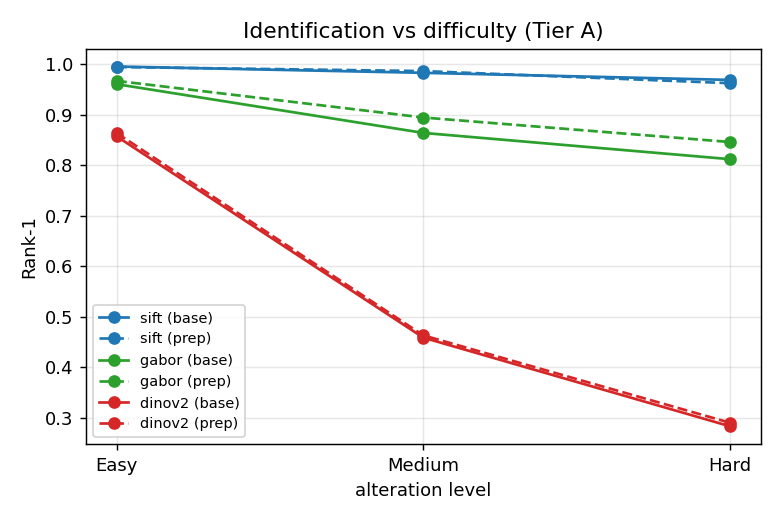
\includegraphics[width=0.62\textwidth]{rank1_by_level.png}
\caption{Rank-1 (Recognition Rate) vs.\ alteration difficulty. Solid = baseline,
dashed = preprocessed.}
\label{fig:rank1}
\end{figure}

\begin{figure}[h]
\centering
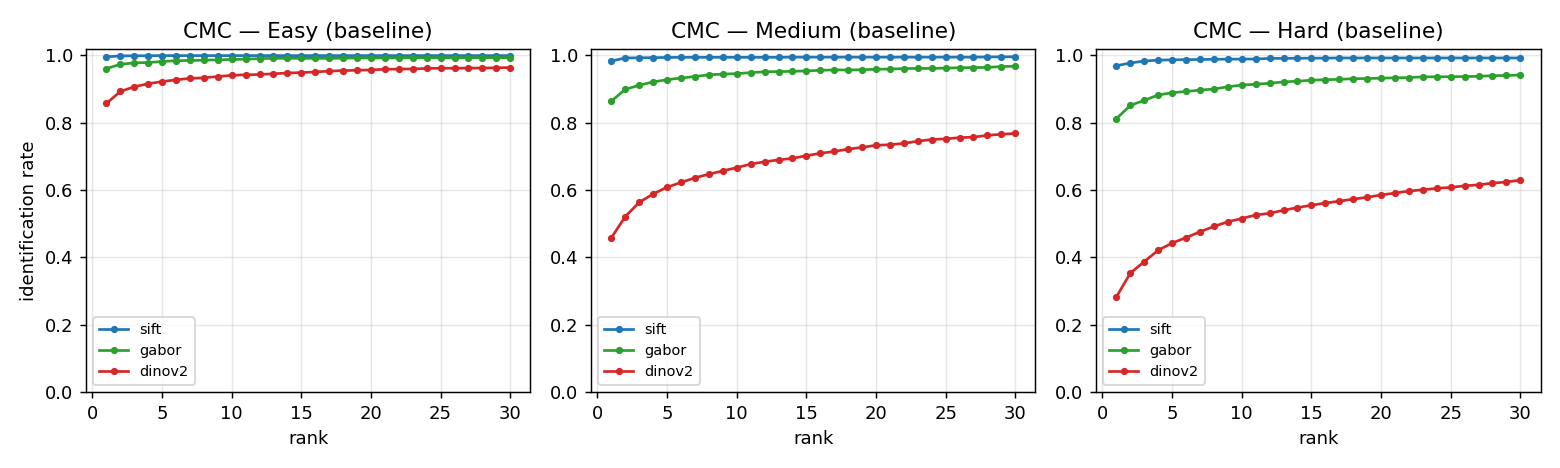
\includegraphics[width=\textwidth]{cmc_by_level.png}
\caption{CMC curves (baseline) for the three models at each difficulty level. SIFT
stays at the top and barely moves; Gabor is intermediate; DINOv2 falls and
diverges as difficulty increases.}
\label{fig:cmc}
\end{figure}

\subsection{Analysis by alteration type}
The per-type breakdown (Table~\ref{tab:alt}) reveals the failure modes.
\textbf{DINOv2 fails on all} hard alterations --- even on a clean cut (Zcut,
$0.305$) that SIFT and Gabor absorb --- because a global embedding cannot tolerate
a missing region. \textbf{Gabor's weakness is obliteration} ($0.654$): texture
statistics degrade when ridges are destroyed, though it stays robust to cutting
($0.981$). \textbf{SIFT is robust to all types} ($\ge0.954$): geometric keypoint
consistency survives rotation, cutting and partial obliteration alike.

\begin{table}[h]
\centering
\caption{Rank-1 by alteration type at the Hard level (baseline).}
\label{tab:alt}
\begin{tabular}{@{}lccc@{}}
\toprule
Hard, Rank-1 & \textbf{SIFT} & \textbf{Gabor} & \textbf{DINOv2} \\
\midrule
CR (rotation)      & 0.954 & 0.802 & 0.234 \\
Obl (obliteration) & 0.964 & 0.654 & 0.310 \\
Zcut (cut)         & 0.990 & 0.981 & 0.305 \\
\bottomrule
\end{tabular}
\end{table}

\subsection{Effect of preprocessing}
The most nuanced result (Table~\ref{tab:prep}, Fig.~\ref{fig:prep}), now
substantiated by the paired McNemar test: the contrast mask \textbf{significantly
helps the texture descriptor (Gabor)}, at every level and strongly so as
difficulty rises (Easy $+0.7$\,pp, $p=0.011$; Medium $+3.0$\,pp and Hard $+3.4$\,pp,
$p<10^{-10}$). For the \textbf{deep embedding (DINOv2)} the small gains are
\textbf{not significant} (Easy/Medium/Hard $p=0.38/0.68/0.52$), and for the
\textbf{keypoint matcher (SIFT)} the effect is likewise \textbf{not significant}
at any level ($p=0.69/0.23/0.15$); sharpening even slightly hurts SIFT at Hard,
plausibly by introducing spurious keypoints that break geometric consistency. A
preprocessing operator devised for facial robustness is therefore not a universal
good: its value is contingent on the downstream representation, and here it is
statistically justified only for Gabor.

\begin{table}[h]
\centering
\caption{$\Delta$Rank-1 from preprocessing (percentage points), with paired
McNemar significance (\textsuperscript{*}$p<0.05$,
\textsuperscript{***}$p<0.001$; ns $=$ not significant). Only Gabor's gains are
statistically significant.}
\label{tab:prep}
\begin{tabular}{@{}lccc@{}}
\toprule
$\Delta$Rank-1 (pp) & Easy & Medium & Hard \\
\midrule
\textbf{Gabor}  & $+0.7$\textsuperscript{*} & $+3.0$\textsuperscript{***} & $+3.4$\textsuperscript{***} \\
\textbf{DINOv2} & $+0.7$~(ns) & $+0.5$~(ns) & $+0.7$~(ns) \\
\textbf{SIFT}   & $-0.1$~(ns) & $+0.4$~(ns) & $-0.6$~(ns) \\
\bottomrule
\end{tabular}
\end{table}

\begin{figure}[h]
\centering
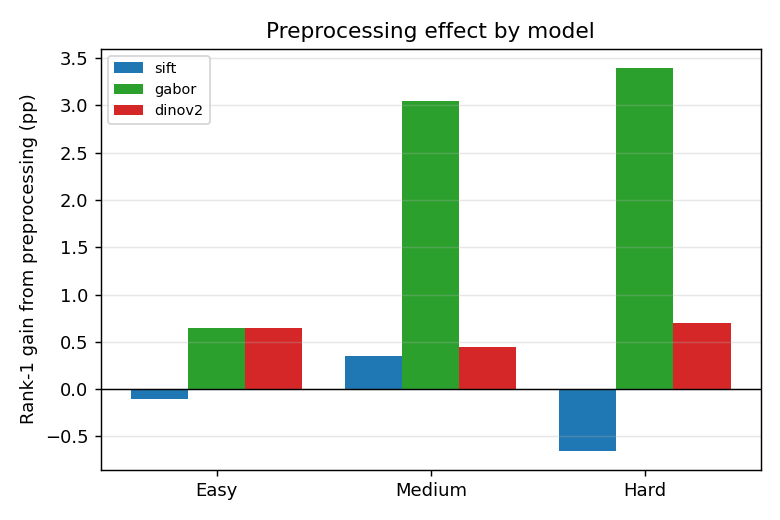
\includegraphics[width=0.60\textwidth]{preprocessing_delta.png}
\caption{Rank-1 gain from preprocessing, by model and level.}
\label{fig:prep}
\end{figure}

\section{Conclusions}
This study compared three frozen fingerprint recognition models on SOCOFing under
increasing alterations, in a closed-set identification setting. The results
overturn common intuition twice. First, the most recent deep model (frozen
DINOv2) is the \emph{worst} and collapses on hard alterations, while the most
classical method (SIFT\,+\,RANSAC) is the \emph{best} and barely degrades: on
altered fingerprints, local geometric robustness beats the global semantics of an
out-of-distribution embedding, and the per-alteration analysis shows global
embeddings are fragile to cuts, texture statistics to obliteration, and geometric
keypoint matching to none of them. Second, the preprocessing pipeline helps one
model (Gabor, increasingly with difficulty), is marginal for another (DINOv2) and
statistically neutral for a third (SIFT), so contrast-enhancement preprocessing
should be validated per model rather than assumed beneficial. The practical
takeaway is that geometric local matching is the safer choice for altered
low-resolution prints.

\begin{thebibliography}{99}

\bibitem{socofing}
Y.~I. Shehu, A.~Ruiz-Garcia, V.~Palade, and A.~James,
``Sokoto Coventry Fingerprint Dataset (SOCOFing),''
\emph{arXiv:1807.10609}, 2018.

\bibitem{lowe2004}
D.~G. Lowe,
``Distinctive image features from scale-invariant keypoints,''
\emph{Int.\ J.\ Computer Vision}, vol.~60, no.~2, pp.~91--110, 2004.

\bibitem{fischler1981}
M.~A. Fischler and R.~C. Bolles,
``Random sample consensus: a paradigm for model fitting with applications to image analysis and automated cartography,''
\emph{Commun.\ ACM}, vol.~24, no.~6, pp.~381--395, 1981.

\bibitem{jain2000}
A.~K. Jain, S.~Prabhakar, L.~Hong, and S.~Pankanti,
``Filterbank-based fingerprint matching,''
\emph{IEEE Trans.\ Image Process.}, vol.~9, no.~5, pp.~846--859, 2000.

\bibitem{dosovitskiy2021}
A.~Dosovitskiy \emph{et al.},
``An image is worth 16x16 words: transformers for image recognition at scale,''
in \emph{ICLR}, 2021. \emph{arXiv:2010.11929}.

\bibitem{oquab2024}
M.~Oquab \emph{et al.},
``DINOv2: learning robust visual features without supervision,''
\emph{TMLR}, 2024. \emph{arXiv:2304.07193}.

\bibitem{nbis}
C.~I. Watson \emph{et al.},
\emph{User's Guide to NIST Biometric Image Software (NBIS)}, NIST, 2007.
(MINDTCT extractor; BOZORTH3 matcher.)

\bibitem{nguyen2018}
D.-L. Nguyen, K.~Cao, and A.~K. Jain,
``Robust minutiae extractor: integrating deep networks and fingerprint domain knowledge,''
in \emph{Int.\ Conf.\ Biometrics (ICB)}, 2018. \emph{arXiv:1712.09401}.

\bibitem{maltoni}
D.~Maltoni, D.~Maio, A.~K. Jain, and S.~Prabhakar,
\emph{Handbook of Fingerprint Recognition}, 2nd ed. Springer, 2009.

\bibitem{mcnemar1947}
Q.~McNemar,
``Note on the sampling error of the difference between correlated proportions or percentages,''
\emph{Psychometrika}, vol.~12, no.~2, pp.~153--157, 1947.

\bibitem{gonzalez}
R.~C. Gonzalez and R.~E. Woods,
\emph{Digital Image Processing}, 4th ed. Pearson, 2018.

\end{thebibliography}

\end{document}
